En esta sección se detalla la construcción de una aplicación de escritorio diseñada para la clasificación de comentarios textuales. Esta aplicación incluye la carga del mejor modelo previamente seleccionado, la matriz de embeddings y el tokenizador correspondiente. La misma permite al usuario ingresar un comentario que será procesado por el modelo clasificador, mostrando el resultado de la clasificación en la pantalla. Esta sección se compone de la siguiente carpeta:

La carpeta clasificadorcnn contiene los siguientes archivos:

\begin{itemize}

\item manipular\_modelo.py: Este archivo incluye funciones para cargar el tokenizador, la matriz de embeddings, ensamblar el modelo clasificador y preprocesar la entrada para realizar la predicción, para más detalles ver la figura \ref{fig:uml12}.

\begin{figure}[h!]
	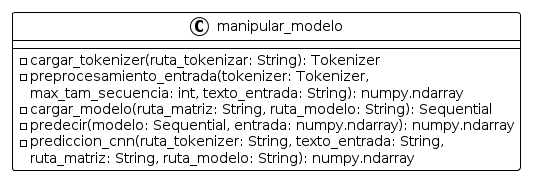
\includegraphics[width=0.8\textwidth]{capitulo5/figuras/fig12.png}
	\caption{Diagrama de clase del archivo manipular\_modelo.py
		\\\textit{Fuente: Elaboracion Propia}}
	\label{fig:uml12}
\end{figure}

\item interfaz.py: Este archivo se encarga de crear la interfaz de usuario, donde se ingresa el comentario a clasificar y se muestran los resultados de la clasificación, para más detalles ver la figura \ref{fig:uml13}.

\begin{figure}[h!]
	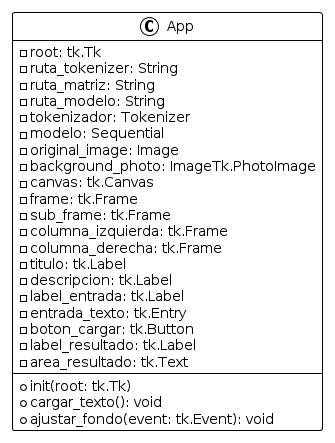
\includegraphics[width=0.5\textwidth]{capitulo5/figuras/fig13.png}
	\caption[Diagrama de clase del archivo interfaz.py]{Diagrama de clase del archivo interfaz.py
		\\\textit{Fuente: Elaboracion Propia}}
	\label{fig:uml13}
\end{figure}

\end{itemize}

Para simplificar la carga del modelo y hacer que los archivos sean más portables, se descompuso el modelo en varias partes:

\begin{itemize}

\item Matriz de embeddings: Se guardó en formato .npy, que es el formato nativo de la librería NumPy de Python, ampliamente utilizada en ciencia de datos y aprendizaje automático para cálculos numéricos. Este formato permite almacenar la matriz de manera eficiente y facilita su carga y uso posterior.

\item Pesos del modelo: Se almacenaron en formato .h5 (HDF5, Hierarchical Data Format version 5), un formato comúnmente usado para manejar datos de alta dimensión y ofrecer almacenamiento jerárquico. Esto permite reutilizar el modelo entrenado sin necesidad de volver a entrenarlo, ya que los pesos se pueden cargar directamente desde el archivo.

\item Tokenizador: Se guardó en formato .pickle, que es un formato binario utilizado en Python para la serialización y deserialización de objetos. Este formato es ideal para almacenar objetos complejos como los tokenizadores, que se usan en aplicaciones de procesamiento de lenguaje natural. La capacidad de .pickle para serializar prácticamente cualquier objeto Python, incluyendo listas, diccionarios y clases personalizadas, hace que sea una opción conveniente para este propósito.

\end{itemize}

